% article example for classicthesis.sty
\documentclass[12pt,a4paper]{article} % KOMA-Script article scrartcl
\usepackage{lipsum}
\usepackage{url}
\usepackage[nochapters]{classicthesis} % nochapters
\usepackage[margin=1in]{geometry}
\usepackage{graphicx}

\begin{document}
    \title{\rmfamily\normalfont\spacedallcaps{Sugarscape with Disease}}
    \author{\spacedlowsmallcaps{Rachel Culpepper, Marissa Sisco, and Tanner Bina}}
    \date{} % no date
    
    \maketitle
    
    
    \section{Project Overview}
    For our final simulation project we extended the sugarscape simulation to include contagious diseases. Our original implementation of sugarscape included 400 agents who collected sugar distributed in two gaussian peaks on a grid. Each agent had a metabolic rate which influenced the amount of sugar they consumed at each time unit. Agents then would move around the grid, collecting sugar and attempting to survive for as long as possible. Agents would move to the most profitable cell within sight and collect the sugar that was at that cell. When old agents died, either from their life span being expended or running out of sugar, new agents were randomly placed in the grid.
    
    Our extension of this simulation included the simulation of immune systems and diseases for each agent. Each agent was given a unique immune system at birth. This immune system was modeled by a long bit string. At the start of the simulation, a set number of diseases were created. Each disease created was randomly assigned a bit string with length between our two set disease length parameters. Each agent was then infected with a set number of these disease upon birth, a process which was repeated anytime an agent was born. 
    
    Diseases increased the metabolism of their host, increasing the likelihood of their death. Whenever a host moved, it had a chance to transmit a diseases to one of its new neighbors. When a disease was transmitted, there was a small set chance that one of the bits in the disease would mutate and change. As well as the mutation of disease, the immune system was capable of mutating to prevent disease. On each time step, the immune system would flip on bit to match more closly with a disease. When the immune system had a substring that matched a disease, the agent became "cured" from that disease and was no longer negatively impacted.
    
    In the next section, we will discuss the parameters which could be edited in our simulation. Following this, we will more closely examine the immune system, the disease structure, and the changes in our event based structure to allow for the addition of diseases. Finally, we will explain some experiments we ran on our simulation and the effects we saw from these experiments.
    
    \section{Parameters}
    To easily edit our simulation, we created a parameter class. Each of these parameters can be edited to effect areas of the simulation. The following is a list of the parameters that can be changed and their base settings:\\
    $MIN\_DISEASE\_LENGTH = 3$ - The minimum length of a disease bitstring.\\
    $MAX\_DISEASE\_LENGTH = 10$ - The maximum length of a disease bitstring.\\
    $DISEASE\_IMPACT = 1$ - The increase in metabolism from one disease.\\
    $IMMUNE\_SYSTEM\_LENGTH = 50$ - The length of the immune system's bitstring.\\
    $NUMBER\_DISEASES = 25$ - The number of diseases generated at the beginning of the simulation.\\
    $BIRTH\_DISEASES = 10$ - The number of diseases given to an agent on birth.\\
    $MUTATION\_PROBABILITY = .01$ - The probability of a disease mutating upon transfer.\\
    $END\_TIME = 100$ - The end time of the simulation.
    
    \section{Immune System}
    Our immune system was modeled by a bitstring, based on the $IMMUNE\_SYSTEM\_LENGTH$ parameter. Whenever the simulation attempted to add a disease to an agent, the immune system was checked to determine if the agent was immune to that disease. An agent was immune to a disease, if there existed a substring in the immune system that matched the bitstring of the disease. If there was such a substring, the agent was immune, and was not infected by the disease. If there was no such substring, the immune system matches the disease to the closest substring to it. Ties are settled by first substring in the immunesystem. At each time step, an immune system updates itself, attempting to "cure" any diseases the agent carried. For each disease, it found the first non matching bit in the substring that the disease matched to. This bit was then switched to be equal to that of the disease. If a disease matched it's substring perfectly after the update, the disease was cured and removed from the host.
    
    \section{Disease}
    Our diseases were modeled by bitstrings. Each bitstring was a random length between our two parameters $MIN\_DISEASE\_LENGTH$ and $MAX\_DISEASE\_LENGTH$. Each disease also increased the metabolism of it's carrier by a value equal to $DISEASE\_IMPACT$. Diseases are static within a host, but can mutate upon transfer to a new host. The probability of mutation is based on $MUTATION\_PROBABILITY$. If a disease mutates, a random bit within its bitstring is switched to the opposite bit. This new form of the disease is then transferred to the new carrier, whereas the old form stays with the original carrier.
    
    \section{Event-Based Changed}
    
    \section{Experimentation}
    The first experiment we tested on our simulation was how mutation probability effects the number of deaths in a simulation, as well as the number of diseases present on average in the end population. An increase in the mutation of disease is related to a decrease in immune systems ability to adapt to diseases, and therefore should be associated with higher death rates and a higher number of disease per agent. The only parameter that was altered in this experiment was the $MUTATION\_PROBABILITY$. All other parameters were set to their default values. The simulation was ran and averaged over 5 runs to determine the values.
    
    \includegraphics[scale = .375]{mutation_prob.png}
    
    As you can see from the above graphs, the number of deaths did not vary quite as expected, except under extremely low mutation probabilities. The average number of diseases, however, varied as we would expect. The fact that the number of deaths did not vary as much as expect under high probability seems to tell us that after a point, an increase in mutation does not increase the deadliness of the disease. The second graph does support our ideas on the decreased ability of an immune system to handle highly mutable diseases.
    
    The second experiment we tested on our simulation was looking at how a change in the max length of disease, changes the end population of our simulation. As we did not want mutation to play a large roll in this simulation, we decreased the mutation probability to $.001$. All other parameters beside $MAX\_DISEASE\_LENGTH$ stayed constant.
    
    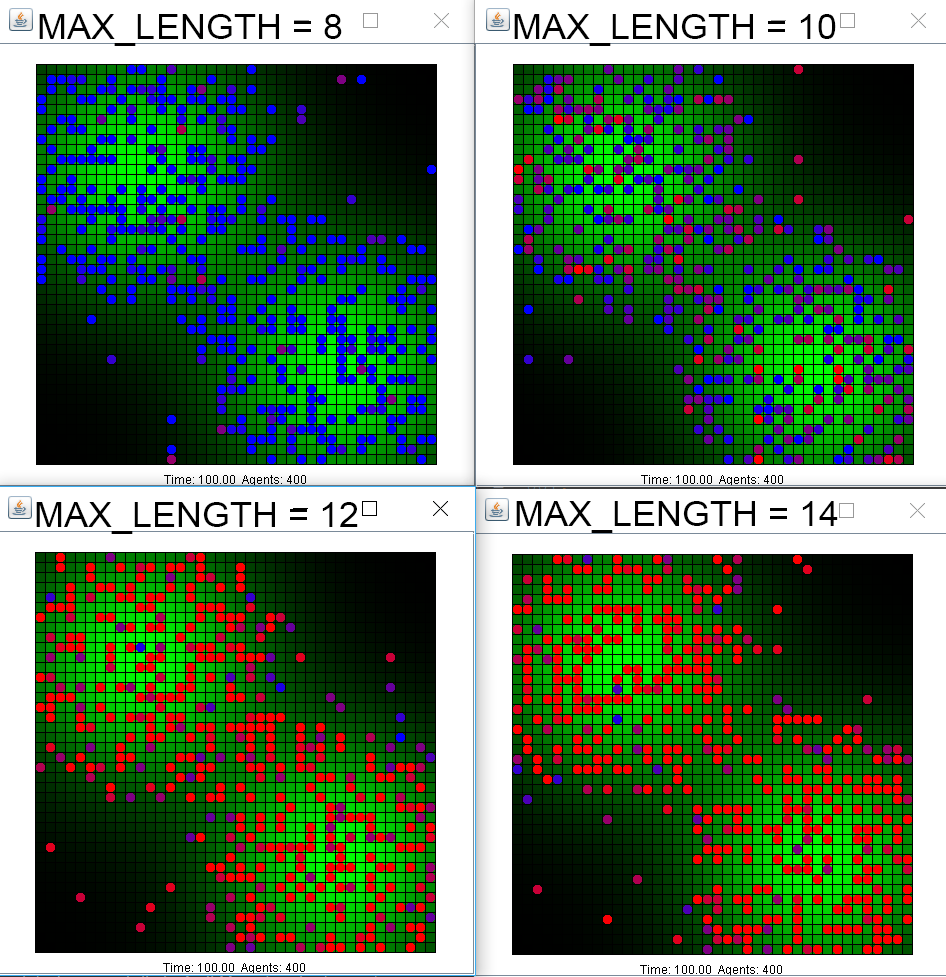
\includegraphics[scale = .45]{Max_length.png}
    
    As you can see by the snapshots of the end state of the simulation, a small variation in the max length of diseases generated has a large impact on the end population. With a small length of only 8, most diseases were cured by the immune system. However, even a length of 12, caused disease to run rampant throughout the population. This large change may be due to the increase probability of overlap between diseases given a longer length. When two diseases overlap, they may fall into an incurable state as they both alter the immune system.
    
    
\end{document}